\tikzstyle{every node}=[circle,draw]
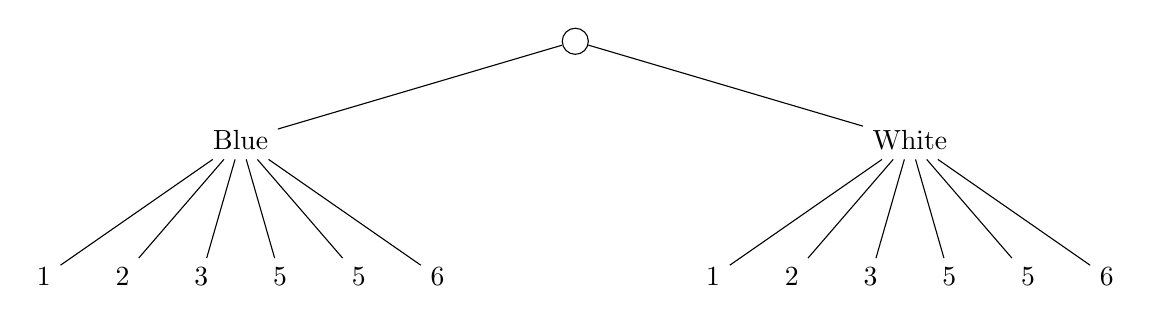
\begin{tikzpicture}[grow=down, sloped,every node/.style = {},level distance=1.5cm,
level 1/.style={sibling distance=8.5cm},
level 2/.style={sibling distance=1cm}]
 \node[circle, draw](dice){}
      child {
            node[above](Blue) {Blue}
            child {
                  node[below] (1) {1}
                  edge from parent
            }
            child {
                   node[below] (2) {2}
                   edge from parent
            }
            child {
                   node[below] (3) {3}
                   edge from parent
            }
            child {
                  node[below] (4) {5}
                  edge from parent
            }
            child {
                  node[below] (5) {5}
                  edge from parent
            }
            child {
                  node[below] (6) {6}
                  edge from parent                 
            }                              
            edge from parent 
      }                       
      child {
              node[above](White) {White}
            child {
                  node[below] (1) {1}
                  edge from parent
            }
            child {
                   node[below] (2) {2}
                   edge from parent
            }
            child {
                   node[below] (3) {3}
                   edge from parent
            }
            child {
                  node[below] (4) {5}
                  edge from parent
            }
            child {
                  node[below] (5) {5}
                  edge from parent
            }
            child {
                  node[below] (6) {6}
                  edge from parent                 
            }                              
              edge from parent
       };
          
% child {node[below](White) {White}
    %             node[below]  {$2$}
%             };    
   
\end{tikzpicture}